\section{Résultats}

\begin{frame}
	\frtt{Ajustement de $\tilde{T}$}
	
	\begin{figure}
	\centering
	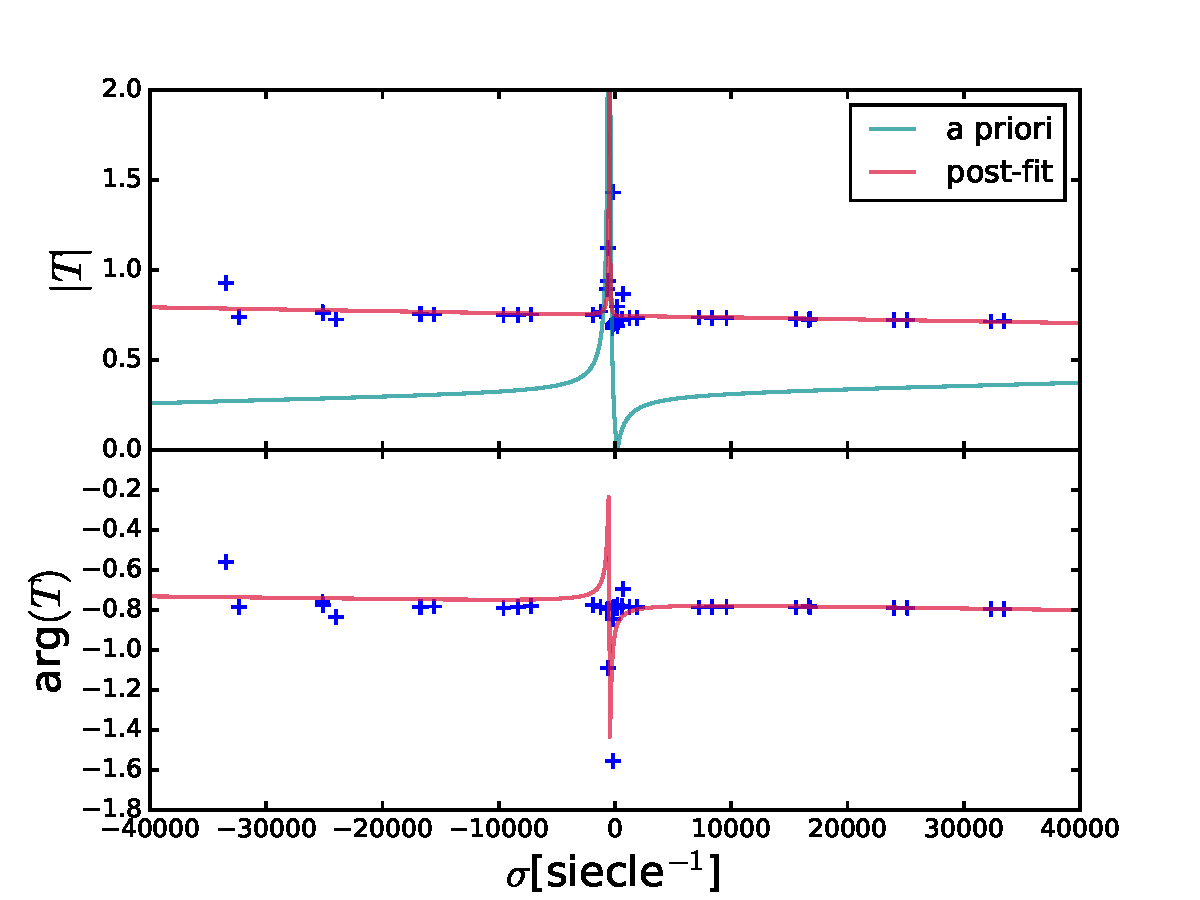
\includegraphics[width=0.9\textwidth]{fit_transfert.pdf}
	\end{figure}

\end{frame}

\begin{frame}
\frtt{Importance et critique des corrections}
\begin{figure}
\begin{tabular}{cccc}
param & a priori & correction post-fit & |correction relat|\\
\hline
$\kappa$ & $1.039e-3$ & $(-1.3+1.6i)e-2$ & $20.3$ \\
%\hline
$\gamma$ & $1.965e-3$ & $(-1.4+1.5i)e-2$ & $10.2$ \\
%\hline
$e$ & $3.257e-3$ &$-0.015+\alert{1.5i}$  & $6.4$ \\
%\hline
$(e_f-\beta)$ & $1.931e-3$ & $(-0.58-1.1i)e-4$ & $6.5e-2$ 
\end{tabular}
\end{figure}
Pour mémoire :
\begin{align*}
\tilde{T}(\sigma) 
     = \frac{e_R\Omega-\sigma}{e_R\Omega} &\left[ \kappa - \frac{A_f}{A}\gamma\right.- \frac{\Omega(e-\kappa)}{\sigma-\frac{A}{A_m}\Omega(e-\kappa)}\\
     &-\left. \frac{A_f}{A_m} \frac{\Omega (e-\gamma)(e_f-\beta)}{\sigma + \Omega(1+ \frac{A}{A_m}(e_f-\beta))}\right]
\end{align*}
\centering
   
    

\end{frame}